\documentclass[
11pt, % The default document font size, options: 10pt, 11pt, 12pt
codirector, % Uncomment to add a codirector to the title page
]{charter} 

\usepackage{enumitem}


% El títulos de la memoria, se usa en la carátula y se puede usar el cualquier lugar del documento con el comando \ttitle
\titulo{Tester para amplificador de fibra óptica} 

% Nombre del posgrado, se usa en la carátula y se puede usar el cualquier lugar del documento con el comando \degreename
\posgrado{Carrera de Especialización en Sistemas Embebidos} 
%\posgrado{Carrera de Especialización en Internet de las Cosas} 
%\posgrado{Carrera de Especialización en Intelegencia Artificial}
%\posgrado{Maestría en Sistemas Embebidos} 
%\posgrado{Maestría en Internet de las cosas}

% Tu nombre, se puede usar el cualquier lugar del documento con el comando \authorname
\autor{Lucas Constantino} 

% El nombre del director y co-director, se puede usar el cualquier lugar del documento con el comando \supname y \cosupname y \pertesupname y \pertecosupname
\director{Nombre del Director}
\pertenenciaDirector{pertenencia} 
% FIXME:NO IMPLEMENTADO EL CODIRECTOR ni su pertenencia
\codirector{John Doe} % para que aparezca en la portada se debe descomentar la opción codirector en el documentclass
\pertenenciaCoDirector{FIUBA}

% Nombre del cliente, quien va a aprobar los resultados del proyecto, se puede usar con el comando \clientename y \empclientename
\cliente{Nicolas Casco}
\empresaCliente{Skyloom Global}

% Nombre y pertenencia de los jurados, se pueden usar el cualquier lugar del documento con el comando \jurunoname, \jurdosname y \jurtresname y \perteunoname, \pertedosname y \pertetresname.
\juradoUno{Nombre y Apellido (1)}
\pertenenciaJurUno{pertenencia (1)} 
\juradoDos{Nombre y Apellido (2)}
\pertenenciaJurDos{pertenencia (2)}
\juradoTres{Nombre y Apellido (3)}
\pertenenciaJurTres{pertenencia (3)}
 
\fechaINICIO{1 de Marzo de 2022}		%Fecha de inicio de la cursada de GdP \fechaInicioName
\fechaFINALPlan{18 de junio de 2022} 		%Fecha de final de cursada de GdP
\fechaFINALTrabajo{15 de mayo de 2022}	%Fecha de defensa pública del trabajo final


\begin{document}

\maketitle
\thispagestyle{empty}
\pagebreak


\thispagestyle{empty}
{\setlength{\parskip}{0pt}
\tableofcontents{}
}
\pagebreak


\section*{Registros de cambios}
\label{sec:registro}


\begin{table}[ht]
\label{tab:registro}
\centering
\begin{tabularx}{\linewidth}{@{}|c|X|c|@{}}
\hline
\rowcolor[HTML]{C0C0C0} 
Revisión & \multicolumn{1}{c|}{\cellcolor[HTML]{C0C0C0}Detalles de los cambios realizados} & Fecha      \\ \hline
1.0	& Creación del documento.						& 01/03/2022 \\ \hline
1.1	& Se completan las secciones 1 a 5 inclusive			& 15/03/2022 \\ \hline
1.2	& Se completan las secciones 6 a 9 inclusive                & 22/03/2022 \\ \hline
%2      & Se completa hasta el punto 7 inclusive
%		  Se puede agregar algo más \newline
%		  En distintas líneas \newline
%		  Así                                                    & dd/mm/aaaa \\ \hline
%3      & Se completa hasta el punto 11 inclusive                & dd/mm/aaaa \\ \hline
%4      & Se completa el plan	                                 & dd/mm/aaaa \\ \hline
\end{tabularx}
\end{table}

\pagebreak



\section*{Acta de constitución del proyecto}
\label{sec:acta}

\begin{flushright}
Buenos Aires, \fechaInicioName
\end{flushright}

\vspace{2cm}

Por medio de la presente se acuerda con el Ing. \authorname\hspace{1px} que su Trabajo Final de la \degreename\hspace{1px} se titulará ``\ttitle'', consistirá esencialmente en el desarrollo y construcción de un dispositivo integrado capaz de monitorear y controlar un amplificador de fibra óptica, y tendrá un presupuesto preliminar estimado de \textcolor{red}{600} hs de trabajo y \textcolor{red}{\$XXX}, con fecha de inicio \fechaInicioName\hspace{1px} y fecha de presentación pública \fechaFinalName.

Se adjunta a esta acta la planificación inicial.

\vfill

% Esta parte se construye sola con la información que hayan cargado en el preámbulo del documento y no debe modificarla
\begin{table}[ht]
\centering
\begin{tabular}{ccc}
\begin{tabular}[c]{@{}c@{}}Ariel Lutenberg \\ Director posgrado FIUBA\end{tabular} & \hspace{2cm} & \begin{tabular}[c]{@{}c@{}}\clientename \\ \empclientename \end{tabular} \vspace{2.5cm} \\ 
\multicolumn{3}{c}{\begin{tabular}[c]{@{}c@{}} \supname \\ Director del Trabajo Final\end{tabular}} \vspace{2.5cm} \\
%\begin{tabular}[c]{@{}c@{}}\jurunoname \\ Jurado del Trabajo Final\end{tabular}     &  & \begin{tabular}[c]{@{}c@{}}\jurdosname\\ Jurado del Trabajo Final\end{tabular}  \vspace{2.5cm}  \\
%\multicolumn{3}{c}{\begin{tabular}[c]{@{}c@{}} \jurtresname\\ Jurado del Trabajo Final\end{tabular}} \vspace{.5cm}                                                                     
\end{tabular}
\end{table}




\section{1. Descripción técnica-conceptual del proyecto a realizar}
\label{sec:descripcion}

Un EDFA (Erbuim-Doped Fiber Amplifier) es un dispositivo optoelectrónico que permite amplificar una señal lumínica transportada mediante una fibra óptica desde una potencia del orden de 1 mW hasta aproximadamente 1 W (unas mil veces). Estos amplificadores se usan particularmente en las bandas L y C del espectro de longitud de onda para compensar las pérdidas en la fibra óptica en comunicaciones de gran distancia.

En general, un EDFA además de contar con una entrada y una salida de fibra óptica tiene un microcontrolador interno encargado de controlar el proceso de amplificación. Para poder comunicarse con el exterior este cuenta con un puerto para la conexión de varias señales, entre ellas la tensión de alimentación (potencia) para la amplificación propiamente dicha y otras señales de entrada y salida tanto analógicas como digitales, que describen el estado del amplificador, valores de ciertos parámetros y una interfaz serie que permite establecer una comunicación con el dispositivo maestro que lo comandará.

El dispositivo a desarrollar debe poder conectarse directamente al puerto de un EDFA del fabricante Nuphoton, proveer la corriente necesaria para que funcione, medirla y presentarle al usuario de forma clara este valor y el resto de los parámetros relevantes recibidos. Para esto debe contar con un display LCD táctil que además permita enviarle comandos al amplificador.

Por otro lado, como el amplificador es un dispositivo muy caro que ademas formará parte de una terminal de comunicación óptica satelital destinada a volar, es imperativo que se tomen las medidas necesarias para evitar dañarlo durante la etapa de integración, tanto mecánica como electricamente. Por dicha razón el dispositivo debe contar con las protecciones eléctricas pertinentes.

En la Figura \ref{fig:diagTester} se presenta el diagrama en bloques del sistema. Se observa que este consta de un microcontrolador como controlador central al cual se encuentran conectados todo el resto de los periféricos e interfaces. Ademas aclara que el EDFA, la PC y la fuente de alimentación externa no forman parte del dispositivo a desarrollar, solamente se encuentran conectados a este mediante algun tipo de interfaz.


\begin{figure}[H]
\centering 
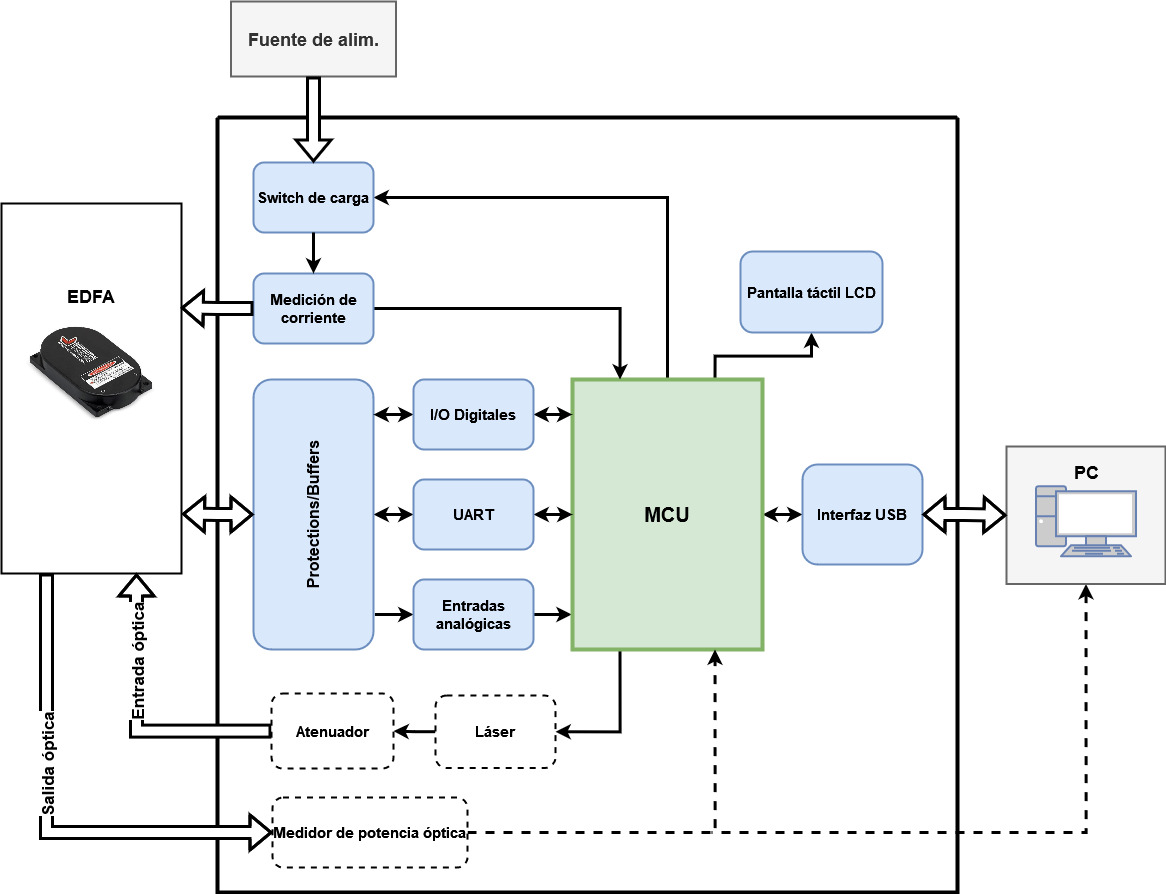
\includegraphics[width=0.75\textwidth]{./Figuras/diagTester.jpg}
\caption{Diagrama en bloques del sistema}
\label{fig:diagTester}
\end{figure}


Si bien el fabricante del EDFA ofrece una placa para establecer una comunicación entre el EDFA y una PC, ademas de ser costosa y no funcionar del todo correctamente, esta no cuenta con la conexión de todas las señales por lo que hace que conocer el estado exacto de todas las señales y parámetros lleve mucho tiempo y requiera una computadora. El presente proyecto se destaca especialmente por incorporar todos los componentes necesarios para poder monitorear y comandar de forma segura este tipo de amplificadores en un solo dispositivo, presentando al usuario los parámetros relevantes del EDFA y su consumo de corriente sin la necesidad de una PC.

Este equipo se enmarca como uno de los denominados Equipamiento Eléctrico de Soporte en Tierra perteneciente al departamento de Ensamble, Integración y Testing de la empresa Skyloom Global y será utilizado tanto durante la etapa de desarrollo como de ensamble de lotes de terminales ópticas satelitales para órbita LEO.


\section{2. Identificación y análisis de los interesados}
\label{sec:interesados}


\begin{table}[ht]
%\caption{Identificación de los interesados}
%\label{tab:interesados}
\begin{tabularx}{\linewidth}{@{}|l|X|X|l|@{}}
\hline
\rowcolor[HTML]{C0C0C0} 
Rol           & Nombre y Apellido & Organización 	& Puesto 	\\ \hline
Cliente       & \clientename      &\empclientename	& Jefe de Proyecto	\\ \hline
Responsable   & \authorname       & FIUBA        	& Alumno 	\\ \hline
Orientador    & \supname	      & \pertesupname 	& Director Trabajo final \\ \hline
%Equipo        & - &              	&        	\\ \hline
Usuario final & -                 & Skyloom Global	& Dpto. de Integración y Testing	\\ \hline
\end{tabularx}
\end{table}

Características de los interesados:
\begin{itemize}
	\item Cliente: es exigente con la presentación del producto y el cumplimiento de sus requerimientos. También puede ayudar a definir los requerimientos.
\end{itemize}


\section{3. Propósito del proyecto}
\label{sec:proposito}

El propósito de este proyecto es desarrollar un dispositivo integrado capaz de proveer al usuario una forma sencilla de monitorear y comandar un EDFA, sin necesidad de usar una computadora. De esta forma el dispositivo se utilizará en dos instancias bien definidas: la primera es durante el desarrollo de nuevos modelos de terminales opticas satelitales y la segunda es durante la integración de grandes lotes para su fabricación en masa.

\section{4. Alcance del proyecto}
\label{sec:alcance}

Este proyecto queda delimitado por:
\begin{itemize}
	\item Diseño y construcción de un dispositivo funcional de un tester que consta de hardware y software.
	\item Diseño y ensamble del PCB del dispositivo.
	\item Integración completa del dispositivo en soporte mecánico.
	\item Verificación funcional del producto final.
	\item Simulación de funcionamiento de hardware mediante software apropiado.
	\item Diseño e implementación de la arquitectura de software del dispositivo.
	\item Diseño e implementación del software a ejecutarse en la PC.
	\item Documentación de diseño para su producción y manual de uso.
\end{itemize}

Por otro lado, queda excluído del presente proyecto:
\begin{itemize}
	\item Fabricación del PCB del dispositivo.
	\item Especificación de las pruebas a ejecutar sobre el amplificador óptico utilizando el dispositivo.
	\item Procesamiento e interpretación de los valores de los parámetros enviados por el EDFA.
	\item Diseño y construcción de la fuente de alimentación externa.
\end{itemize}


\section{5. Supuestos del proyecto}
\label{sec:supuestos}

Para el desarrollo del presente proyecto se supone que:
\begin{itemize}
	\item El cliente proveerá una versión inicial de la placa del dispositivo final para desarrollo.
	\item Se podrá contar con los insumos necesarios en tiempo y forma.
	\item El cliente posee las instalaciones e instrumental necesario para realizar mediciones y ensayos.
	\item Se dispondrá del tiempo necesario para el desarrollo del proyecto.
	\item Se cuenta con toda la información técnica acerca del amplificador óptico, sus parámetros y funcionamiento.
	\item Se contará con un EDFA o con una placa electrónica que simule su comportamiento.
	\item El contexto macroeconómico permitirá mantener al proyecto económicamente viable durante toda su duración.
	\item El dispositivo le seguirá siendo necesario al cliente al momento de la finalización del proyecto.
\end{itemize}

\section{6. Requerimientos}
\label{sec:requerimientos}

Los requerimientos del proyecto se definieron luego de acordarlos con el cliente y considerando las sugerencias de los posibles usuarios finales. Estos se detallan a continuación, agrupados en distintas secciones y en orden de prioridad decreciente.

\begin{enumerate}
	\item Requerimientos generales
		\begin{enumerate}
			\item Fecha de entrega del proyecto terminado: A definir
			\item Todos los componentes del dispositivo, a excepción de la fuente de alimentación, deben estar montados sobre una carcasa de material no conductor.
			\item El dispositivo debe poder conectarse a la red de 110V/60Hz mediante una fuente de alimentación externa.
			\item El dispositivo, sin la fuente de alimentaciön externa, no debe pesar mas de 750 g y no debe tener mas de 15 cm de largo, 10 cm de ancho y 6 cm de alto.
			\item El dispositivo debe conectarse al EDFA mediante un cable con conectores Micro-D.
		\end{enumerate}
	\item Requerimientos funcionales
		\begin{enumerate}
			\item Requerimientos de hardware
				\begin{enumerate}[label*=\arabic*.]
					\item Todas las señales eléctricas entrantes y salientes del EDFA deben estar aisladas y protegidas contra descargas electrostáticas.
					\item El dispositivo debe contar con una pantalla táctil y mostrar en ella el estado de todas las señales del EDFA y los valores de sus parámetros.
					\item El dispositivo debe poder medir el consumo de corriente del EDFA con una precisión del 10\%.
					\item El dispositivo debe desconectar la alimentación del EDFA de forma automática si el consumo de corriente supera el valor establecido por el usuario. Este valor debe ser configurable por el usuario mediante la pantalla táctil.
					\item El dispositivo debe poder medir el nivel de tensión de alimentación del EDFA con una precisión del 10\%.
					\item El dispositivo debe desconectar la alimentación del EDFA de forma automática si el nivel de tensión cae por debajo del valor establecido por el usuario. Este valor debe ser configurable por el usuario mediante la pantalla táctil.
					\item El dispositivo debe poder conectarse a una computadora mediante USB.
				\end{enumerate}
			\item Requerimientos de firmware
				\begin{enumerate}[label*=\arabic*.]
					\item El dispositivo debe utilizar un sistema operativo en tiempo real.
					\item El dispositivo debe establecer una comunicación con el EDFA para el envío de comandos mediante una interfaz UART.
					\item Cuando el dispositivo se encuentra conectado a una computadora el usuario debe poder, mediante una consola, configurar los mismos parámetros que en la pantalla táctil y además, establecer una comunicación directa con el EDFA.
					\item El dispositivo debe actualizar la información mostrada en la pantalla al menos cada 0.5 segundos.
					\item El dispositivo debe interpretar las señales analógicas de entrada, procesarlas y mostrarlas en la pantalla.
				\end{enumerate}
		\end{enumerate}
	\item Requerimientos no funcionales
		\begin{enumerate}
			\item Se deberá generar la documenatación correspondiente.
			\item El dispositivo debe ser apto para su uso en una sala limpia.
			\item El dispositivo no debe generar ni emanar ningún tipo de partículas o residuo.
			\item El dispositivo debe cumplir con la normativa vigente de compatibilidad electromagnética.
			\item El dispositivo no debe generar altas temperaturas.
		\end{enumerate}
	\item Requerimientos de testing
		\begin{enumerate}
			\item Test de consumo de corriente del EDFA.
			\item Test de desconexión de alimentación del EDFA por sobrecorriente.
			\item Test de comunicación UART con EDFA.
			\item Test de nivel de tensión de alimentación del EDFA.
			\item Test de desconexión de alimentación del EDFA por caída de tensión.
			\item Test de uso del dispositivo mediante una computadora.
		\end{enumerate}
	\item Requerimientos opcionales
		\begin{enumerate}
			\item El dispositivo podría contar con un software de PC con interfaz gráfica para el manejo de la comunicación con el EDFA y el monitoreo de señales.
		\end{enumerate}
\end{enumerate}

% Faltaria poner los requerimientos de regulaciones y normas vigentes

\section{7. Historias de usuarios (\textit{Product backlog})}
\label{sec:backlog}

Se dará una visión de las funcionalidades esperadas por los distintos usuarios del producto. A cada
historia se le asocia un grado de ponderación de acuerdo a un criterio definido y una prioridad
respecto al resto.


Para la ponderación se usarán tres niveles: 1, 3 y 7. 
Para la prioridad se usará de 1 a 5, siendo 1 la prioridad mas baja.

\begin{enumerate}
	\item Como ingeniero de desarrollo desearía poder saber el consumo de corriente del EDFA cuando está funcionando activamente sobre una señal óptica para poder calcular su eficiencia.
	\begin{itemize}
		\item Ponderación: 7
		\item Prioridad: 3
	\end{itemize}
	\item Como técnico de integración desearía poder probar todas las señales del EDFA rápidamente para realizar una aceptación de lote en poco tiempo.
	\begin{itemize}
		\item Ponderación: 7
		\item Prioridad: 5
	\end{itemize}
	\item Como ingeniero de desarrollo desearía poder contar con un dispositivo integrado que indique todos los parámetros internos del EDFA para poder monitorear su performance, sin necesidad de usar una computeadora u otro instrumento.
	\begin{itemize}
		\item Ponderación: 3
		\item Prioridad: 4
	\end{itemize}
	\item Como técnico de integración desearía poder enviarle comandos al EDFA para simular que se encuentra conectado a un dispositivo que lo controla, y asi observar su comportamiento.
	\begin{itemize}
		\item Ponderación: 1
		\item Prioridad: 2
	\end{itemize}
	\item Como ingeniero de desarrollo desearía que el dispositivo cuente con las medidas de protección necesarias tanto como para evitar dañar equipos de vuelo como para poder utilizarlo dentro de una sala limpia.
	\begin{itemize}
		\item Ponderación: 3
		\item Prioridad: 2
	\end{itemize}
\end{enumerate}

\section{8. Entregables principales del proyecto}
\label{sec:entregables}

Se incluyen los siguientes entregables:

\begin{itemize}
	\item Manual de uso del dispositivo
	\item Diagramas de circuitos esquemáticos
	\item Código fuente del firmware
	\item Reporte de ensayos
	\item Producto final funcional
	\item Memoria del proyecto
\end{itemize}

\section{9. Desglose del trabajo en tareas}
\label{sec:wbs}

Se presenta a continuación el WBS del proyecto mediante una lista indexada, detallando las actividades a realizar en cada sección y su duración correspondiente.

\begin{enumerate}
\item Planificación del proyecto (50 hs)
	\begin{enumerate}
	\item Definición de alcance y requerimientos con el cliente (12 hs)
	\item Análisis de factibilidad técnico-económica (8 hs)
	\item Confección del plan de trabajo (30 hs)
	\end{enumerate}
\item Análisis preliminar (32 hs)
	\begin{enumerate}
	\item Estudio detallado del funcionamiento del EDFA (12 hs)
	\item Elección del microcontrolador (8 hs)
	\item Selección de los principales componentes a utilizar (12 hs)
	\end{enumerate}
\item Diseño general del dispositivo (50 hs)
	\begin{enumerate}
	\item Construcción de diagrama en bloques (12 hs)
	\item Definición de interfaces (6 hs)
	\item Diseño y fabricación de placa de desarrollo (32 hs)
	\end{enumerate}
\item Diseño de hardware (122 hs)
	\begin{enumerate}
	\item Diseño del diagrama esquemático (30 hs)
	\item Diseño del PCB (24 hs)
	\item Ensamble del PCB (12 hs)
	\item Puesta en marcha del PCB (12 hs)
	\item Ejecución de retrabajos del PCB (6 hs)
	\item Diseño de la carcasa (20 hs)
	\item Impresión de la carcasa (12 hs)
	\item Integración y montaje del dispositivo completo (6 hs)
	\end{enumerate}
\item Diseño de firmware (140 hs)
	\begin{enumerate}
	\item Definición de la arquitectura (14 hs)
	\item Modularización del código (20 hs)
	\item Desarrollo de la interfaz de usuario en pantalla táctil (30 hs)
	\item Desarrollo del monitoreo y protección de corriente (10 hs)
	\item Desarrollo del monitoreo y protección de tensión (10 hs)
	\item Desarrollo de la interfaz UART (26 hs)
	\item Desarrollo de la interfaz USB (30 hs)
	\end{enumerate}
\item Verificación y validación (146 hs)
	\begin{enumerate}
	\item Pruebas de campo (32 hs)
	\item Pruebas de la interfaz de usuario (14 hs)
	\item Pruebas del monitor de corriente (10 hs)
	\item Pruebas de la protección de corriente (10 hs)
	\item Pruebas del monitor de tensión (10 hs)
	\item Pruebas de la protección de tensión (10 hs)
	\item Pruebas de la interfaz UART (20 hs)
	\item Pruebas de la interfaz USB (20 hs)
	\item Corrección de errores del firmware (20 hs)
	\end{enumerate}
\item Documentación (102 hs)
	\begin{enumerate}
	\item Elaboración del manual de usuario (32 hs)
	\item Elaboración de la memoria técnica (40 hs)
	\item Elaboración de la presentación pública del proyecto (30 hs)
	\end{enumerate}
\end{enumerate}

Cantidad total de horas: (642 hs)

\section{10. Diagrama de Activity On Node}
\label{sec:AoN}

\begin{consigna}{red}
Armar el AoN a partir del WBS definido en la etapa anterior. 

%La figura \ref{fig:AoN} fue elaborada con el paquete latex tikz y pueden consultar la siguiente referencia \textit{online}:

%\url{https://www.overleaf.com/learn/latex/LaTeX_Graphics_using_TikZ:_A_Tutorial_for_Beginners_(Part_3)\%E2\%80\%94Creating_Flowcharts}

\end{consigna}

\begin{figure}[H]
\centering 
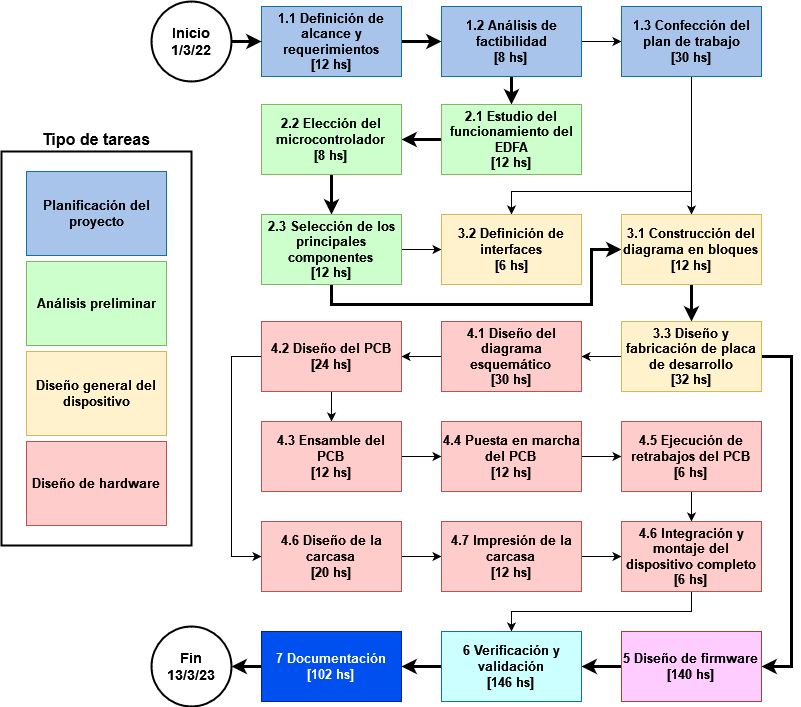
\includegraphics[width=.8\textwidth]{./Figuras/AoN.png}
\caption{Diagrama en \textit{Activity on Node}}
\label{fig:AoN}
\end{figure}

Indicar claramente en qué unidades están expresados los tiempos.
De ser necesario indicar los caminos semicríticos y analizar sus tiempos mediante un cuadro.
Es recomendable usar colores y un cuadro indicativo describiendo qué representa cada color, como se muestra en el siguiente ejemplo:



\section{11. Diagrama de Gantt}
\label{sec:gantt}

\begin{consigna}{red}

Existen muchos programas y recursos \textit{online} para hacer diagramas de gantt, entre los cuales destacamos:

\begin{itemize}
\item Planner
\item GanttProject
\item Trello + \textit{plugins}. En el siguiente link hay un tutorial oficial: \\ \url{https://blog.trello.com/es/diagrama-de-gantt-de-un-proyecto}
\item Creately, herramienta online colaborativa. \\\url{https://creately.com/diagram/example/ieb3p3ml/LaTeX}
\item Se puede hacer en latex con el paquete \textit{pgfgantt}\\ \url{http://ctan.dcc.uchile.cl/graphics/pgf/contrib/pgfgantt/pgfgantt.pdf}
\end{itemize}

Pegar acá una captura de pantalla del diagrama de Gantt, cuidando que la letra sea suficientemente grande como para ser legible. 
Si el diagrama queda demasiado ancho, se puede pegar primero la ``tabla'' del Gantt y luego pegar la parte del diagrama de barras del diagrama de Gantt.

Configurar el software para que en la parte de la tabla muestre los códigos del EDT (WBS).\\
Configurar el software para que al lado de cada barra muestre el nombre de cada tarea.\\
Revisar que la fecha de finalización coincida con lo indicado en el Acta Constitutiva.

En la figura \ref{fig:gantt}, se muestra un ejemplo de diagrama de gantt realizado con el paquete de \textit{pgfgantt}. En la plantilla pueden ver el código que lo genera y usarlo de base para construir el propio.

\begin{figure}[htbp]
\begin{center}
\begin{ganttchart}{1}{12}
  \gantttitle{2020}{12} \\
  \gantttitlelist{1,...,12}{1} \\
  \ganttgroup{Group 1}{1}{7} \\
  \ganttbar{Task 1}{1}{2} \\
  \ganttlinkedbar{Task 2}{3}{7} \ganttnewline
  \ganttmilestone{Milestone o hito}{7} \ganttnewline
  \ganttbar{Final Task}{8}{12}
  \ganttlink{elem2}{elem3}
  \ganttlink{elem3}{elem4}
\end{ganttchart}
\end{center}
\caption{Diagrama de gantt de ejemplo}
\label{fig:gantt}
\end{figure}


\begin{landscape}
\begin{figure}[htpb]
\centering 
\includegraphics[height=.85\textheight]{./Figuras/Gantt-2.png}
\caption{Ejemplo de diagrama de Gantt rotado}
\label{fig:diagGantt}
\end{figure}

\end{landscape}

\end{consigna}


\section{12. Presupuesto detallado del proyecto}
\label{sec:presupuesto}

\begin{consigna}{red}
Si el proyecto es complejo entonces separarlo en partes:
\begin{itemize}
	\item Un total global, indicando el subtotal acumulado por cada una de las áreas.
	\item El desglose detallado del subtotal de cada una de las áreas.
\end{itemize}

IMPORTANTE: No olvidarse de considerar los COSTOS INDIRECTOS.

\end{consigna}

\begin{table}[htpb]
\centering
\begin{tabularx}{\linewidth}{@{}|X|c|r|r|@{}}
\hline
\rowcolor[HTML]{C0C0C0} 
\multicolumn{4}{|c|}{\cellcolor[HTML]{C0C0C0}COSTOS DIRECTOS} \\ \hline
\rowcolor[HTML]{C0C0C0} 
Descripción &
  \multicolumn{1}{c|}{\cellcolor[HTML]{C0C0C0}Cantidad} &
  \multicolumn{1}{c|}{\cellcolor[HTML]{C0C0C0}Valor unitario} &
  \multicolumn{1}{c|}{\cellcolor[HTML]{C0C0C0}Valor total} \\ \hline
 &
  \multicolumn{1}{c|}{} &
  \multicolumn{1}{c|}{} &
  \multicolumn{1}{c|}{} \\ \hline
 &
  \multicolumn{1}{c|}{} &
  \multicolumn{1}{c|}{} &
  \multicolumn{1}{c|}{} \\ \hline
\multicolumn{1}{|l|}{} &
   &
   &
   \\ \hline
\multicolumn{1}{|l|}{} &
   &
   &
   \\ \hline
\multicolumn{3}{|c|}{SUBTOTAL} &
  \multicolumn{1}{c|}{} \\ \hline
\rowcolor[HTML]{C0C0C0} 
\multicolumn{4}{|c|}{\cellcolor[HTML]{C0C0C0}COSTOS INDIRECTOS} \\ \hline
\rowcolor[HTML]{C0C0C0} 
Descripción &
  \multicolumn{1}{c|}{\cellcolor[HTML]{C0C0C0}Cantidad} &
  \multicolumn{1}{c|}{\cellcolor[HTML]{C0C0C0}Valor unitario} &
  \multicolumn{1}{c|}{\cellcolor[HTML]{C0C0C0}Valor total} \\ \hline
\multicolumn{1}{|l|}{} &
   &
   &
   \\ \hline
\multicolumn{1}{|l|}{} &
   &
   &
   \\ \hline
\multicolumn{1}{|l|}{} &
   &
   &
   \\ \hline
\multicolumn{3}{|c|}{SUBTOTAL} &
  \multicolumn{1}{c|}{} \\ \hline
\rowcolor[HTML]{C0C0C0}
\multicolumn{3}{|c|}{TOTAL} &
   \\ \hline
\end{tabularx}%
\end{table}


\section{13. Gestión de riesgos}
\label{sec:riesgos}

\begin{consigna}{red}
a) Identificación de los riesgos (al menos cinco) y estimación de sus consecuencias:
 
Riesgo 1: detallar el riesgo (riesgo es algo que si ocurre altera los planes previstos de forma negativa)
\begin{itemize}
	\item Severidad (S): mientras más severo, más alto es el número (usar números del 1 al 10).\\
	Justificar el motivo por el cual se asigna determinado número de severidad (S).
	\item Probabilidad de ocurrencia (O): mientras más probable, más alto es el número (usar del 1 al 10).\\
	Justificar el motivo por el cual se asigna determinado número de (O). 
\end{itemize}   

Riesgo 2:
\begin{itemize}
	\item Severidad (S): 
	\item Ocurrencia (O):
\end{itemize}

Riesgo 3:
\begin{itemize}
	\item Severidad (S): 
	\item Ocurrencia (O):
\end{itemize}


b) Tabla de gestión de riesgos:      (El RPN se calcula como RPN=SxO)

\begin{table}[htpb]
\centering
\begin{tabularx}{\linewidth}{@{}|X|c|c|c|c|c|c|@{}}
\hline
\rowcolor[HTML]{C0C0C0} 
Riesgo & S & O & RPN & S* & O* & RPN* \\ \hline
       &   &   &     &    &    &      \\ \hline
       &   &   &     &    &    &      \\ \hline
       &   &   &     &    &    &      \\ \hline
       &   &   &     &    &    &      \\ \hline
       &   &   &     &    &    &      \\ \hline
\end{tabularx}%
\end{table}

Criterio adoptado: 
Se tomarán medidas de mitigación en los riesgos cuyos números de RPN sean mayores a...

Nota: los valores marcados con (*) en la tabla corresponden luego de haber aplicado la mitigación.

c) Plan de mitigación de los riesgos que originalmente excedían el RPN máximo establecido:
 
Riesgo 1: plan de mitigación (si por el RPN fuera necesario elaborar un plan de mitigación).
  Nueva asignación de S y O, con su respectiva justificación:
  - Severidad (S): mientras más severo, más alto es el número (usar números del 1 al 10).
          Justificar el motivo por el cual se asigna determinado número de severidad (S).
  - Probabilidad de ocurrencia (O): mientras más probable, más alto es el número (usar del 1 al 10).
          Justificar el motivo por el cual se asigna determinado número de (O).

Riesgo 2: plan de mitigación (si por el RPN fuera necesario elaborar un plan de mitigación).
 
Riesgo 3: plan de mitigación (si por el RPN fuera necesario elaborar un plan de mitigación).

\end{consigna}


\section{14. Gestión de la calidad}
\label{sec:calidad}

\begin{consigna}{red}
Para cada uno de los requerimientos del proyecto indique:
\begin{itemize} 
\item Req \#1: copiar acá el requerimiento.

\begin{itemize}
	\item Verificación para confirmar si se cumplió con lo requerido antes de mostrar el sistema al cliente. Detallar 
	\item Validación con el cliente para confirmar que está de acuerdo en que se cumplió con lo requerido. Detallar  
\end{itemize}

\end{itemize}

Tener en cuenta que en este contexto se pueden mencionar simulaciones, cálculos, revisión de hojas de datos, consulta con expertos, mediciones, etc.  Las acciones de verificación suelen considerar al entregable como ``caja blanca'', es decir se conoce en profundidad su funcionamiento interno.  En cambio, las acciones de validación suelen considerar al entregable como ``caja negra'', es decir, que no se conocen los detalles de su funcionamiento interno.

\end{consigna}

\section{15. Procesos de cierre}    
\label{sec:cierre}

\begin{consigna}{red}
Establecer las pautas de trabajo para realizar una reunión final de evaluación del proyecto, tal que contemple las siguientes actividades:

\begin{itemize}
	\item Pautas de trabajo que se seguirán para analizar si se respetó el Plan de Proyecto original:
	 - Indicar quién se ocupará de hacer esto y cuál será el procedimiento a aplicar. 
	\item Identificación de las técnicas y procedimientos útiles e inútiles que se emplearon, y los problemas que surgieron y cómo se solucionaron:
	 - Indicar quién se ocupará de hacer esto y cuál será el procedimiento para dejar registro.
	\item Indicar quién organizará el acto de agradecimiento a todos los interesados, y en especial al equipo de trabajo y colaboradores:
	  - Indicar esto y quién financiará los gastos correspondientes.
\end{itemize}

\end{consigna}


\end{document}
